\documentclass[8pt,a4paper,compress,handout]{beamer}

\usepackage{/home/siyer/lib/slides}

\title{Searching and Sorting}
\date{}

\begin{document}
\begin{frame}
\vfill
\titlepage
\end{frame}

\begin{frame}
\frametitle{Outline}
\tableofcontents
\end{frame}

\section{Performance}
\begin{frame}[fragile]
\emph{Algorithms} are methods for solving computational problems

\bigskip

\emph{Data structures} are schemes for arranging data, amenable to efficient processing by algorithms

\bigskip

The performance characteristics of a program is determined by
\begin{itemize}
\item its \emph{time complexity}, ie, how long it takes; and 

\item its \emph{space complexity}, ie, how much memory it needs
\end{itemize}
\end{frame}

\begin{frame}[fragile]
The running time of a program is determined by the cost of executing each statement, and the frequency of execution of each statement

\bigskip

Running time is expressed using an \emph{order-of-growth} function of the problem size $N$, without any lower-order terms or constant coefficients

\bigskip

Order-of-growth classifications
\begin{center}
\begin{tabular}{cccc}
description & function & code description & example \\ \hline
constant & 1 & statement & add two numbers \\
logarithmic & $\log N$ & divide in half & binary search \\
linear & $N$ & loop & find the maximum \\
linearithmic & $N\log N$ & divide and conquer & merge sort \\
quadratic & $N^2$ & double loop & check all pairs \\
cubic & $N^3$ & triple loop & check all triples \\
exponential & $2^N$ & exhaustive search & check all subsets
\end{tabular} 
\end{center}
\begin{center}
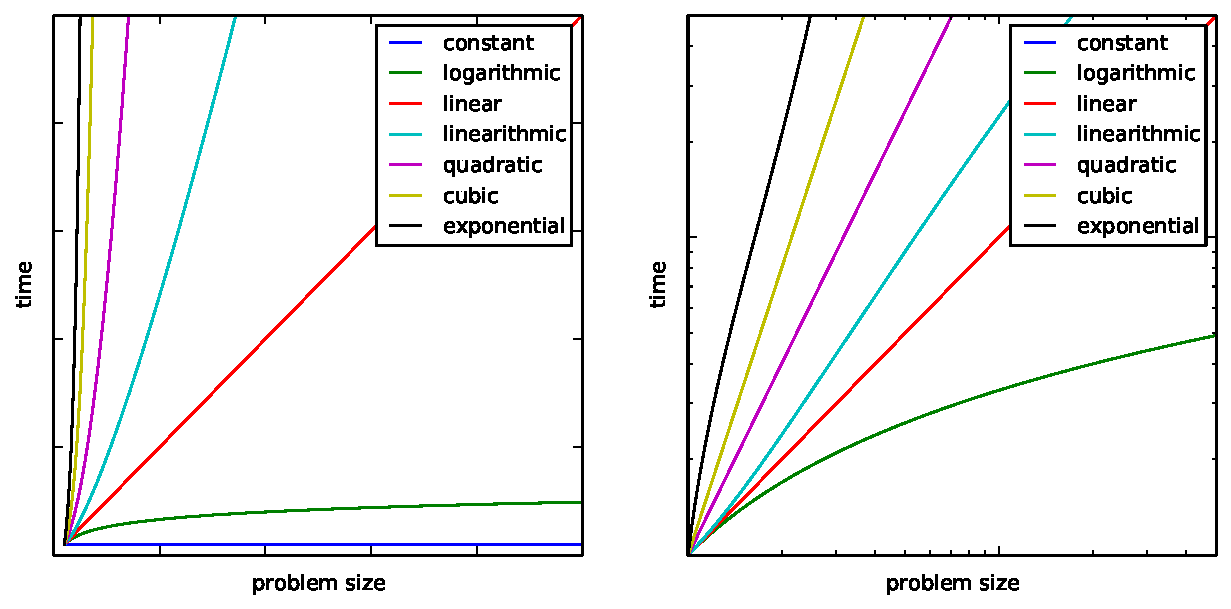
\includegraphics[scale=0.25]{{./figures/order_of_growth}.pdf}
\end{center}
\end{frame}

\begin{frame}[fragile]
The sizes of objects of built-in types differ from system to system, so the sizes of data types that we create also differ accordingly

\bigskip

The function call \lstinline{sys.getsizeof(x)} returns the number of bytes that a built-in object \lstinline{x} consumes on a particular system

\bigskip

Sizes of built-in objects on a typical system
\begin{center}
\begin{tabular}{cc}
object & size in bytes \\ \hline
integer & 24 \\ 
float & 24 \\ 
boolean & 24 \\ 
string of $n$ characters & $40 + n$ \\
list of $n$ integers & $72 + 8n + 24n = 72 + 32n$ \\
$m$-by-$n$ list of integers & $72 + 8m + m(72 + 32n) = 72 + 80m + 32mn$ \\
user-defined & hundreds of bytes, at least
\end{tabular} 
\end{center}
\end{frame}

\section{Searching}
\begin{frame}[fragile]
The \emph{search problem} involves searching for a key in a collection of $N$ keys

\bigskip

Linear search
\begin{lstlisting}[language=Python]
def search(key, a):
    for i, v in enumerate(a):
        if key == v:
            return i
    return -1
\end{lstlisting}

\bigskip

Binary search

\begin{minipage}{150pt}
\begin{center}
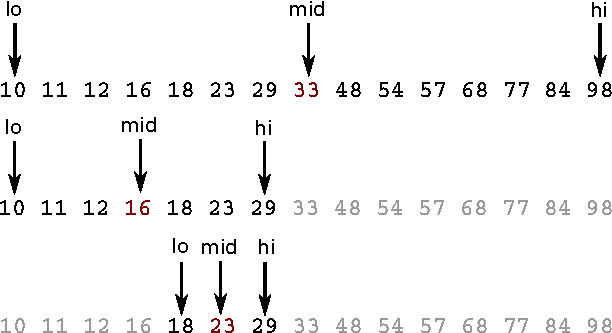
\includegraphics[scale=0.4]{./figures/bs1.pdf}

\smallskip

\tiny successful search for the key 23
\end{center}
\end{minipage}
\begin{minipage}{150pt}%
\hfill
\begin{center}
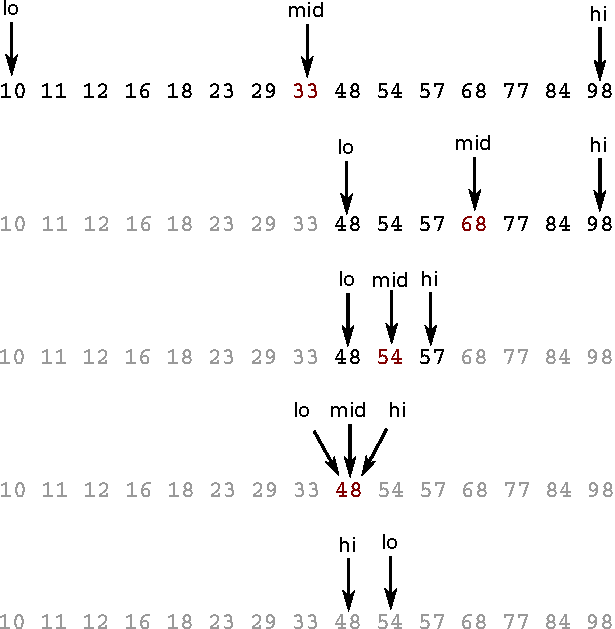
\includegraphics[scale=0.4]{./figures/bs2.pdf}

\smallskip

\tiny unsuccessful search for the key 50
\end{center}
\end{minipage}
\end{frame}

\begin{frame}[fragile]
\begin{framed}
\tiny binarysearch.py: Accepts as a command-line argument a string which is the name of a whitelist file, and writes to standard output the keys in standard input that are not in the whitelist file.
\end{framed}

\begin{lstlisting}[language=Python]
import instream
import stdio
import sys

def _search(key, a, lo, hi):
    if hi <= lo:
        return -1
    mid = (lo + hi) // 2
    if key < a[mid]:
        return _search(key, a, lo, mid)
    elif a[mid] < key:
        return _search(key, a, mid + 1, hi)
    else:
        return mid

def search(key, a):
    return _search(key, a, 0, len(a))

def main():
    inStream = instream.InStream(sys.argv[1])
    a = inStream.readAllStrings()
    while not stdio.isEmpty():
        key = stdio.readString()
        if search(key, a) < 0:
            stdio.writeln(key)

if __name__ == '__main__':
    main()
\end{lstlisting}
\end{frame}

\begin{frame}[fragile]
\begin{lstlisting}[language={}]
$ more emails.txt 
bob@office
carl@beach
marvin@spam
bob@office
bob@office
mallory@spam
dave@boat
eve@airport
alice@home
\end{lstlisting}

\begin{lstlisting}[language={}]
$ more white.txt
alice@home
bob@office
carl@beach
dave@boat
\end{lstlisting}

\begin{lstlisting}[language={}]
$ python binarysearch.py white.txt < emails.txt 
marvin@spam
mallory@spam
eve@airport
\end{lstlisting}
\end{frame}

\section{Sorting}
\begin{frame}[fragile]
The \emph{sort problem} involves rearranging a sequence of objects so as to put them in some logical order

\bigskip

\emph{Insertion sort} is similar to sorting a bridge hand --- consider the cards one at a time, inserting each into its proper place among those already considered
\begin{center}
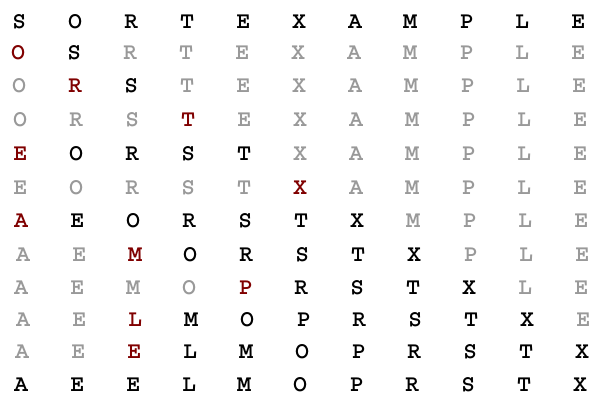
\includegraphics[scale=0.3]{figures/insertion.png}

\smallskip

\tiny insertion sort
\end{center}
\end{frame}

\begin{frame}[fragile]
\begin{framed}
\tiny insertion.py: Reads strings from standard input, sorts them into increasing order, and writes them to standard output.
\end{framed}

\begin{lstlisting}[language=Python]
import stdio
import sys

def exchange(a, i, j):
    a[i], a[j] = a[j], a[i]

def sort(a):
    n = len(a)
    for i in range(1, n):
        j = i
        while (j > 0) and (a[j] < a[j - 1]):
            exchange(a, j - 1, j)
            j -= 1

def main():
    a = stdio.readAllStrings()
    sort(a)
    for s in a:
        stdio.write(s + ' ')
    stdio.writeln()

if __name__ == '__main__':
    main()
\end{lstlisting}

\begin{lstlisting}[language={}]
$ more tiny.txt 
the and was his you tom but for had him
\end{lstlisting}

\begin{lstlisting}[language={}]
$ python insertion.py < tiny.txt 
and but for had him his the tom was you 
\end{lstlisting}
\end{frame}

\begin{frame}[fragile]
\emph{Merge sort} is based on a simple operation known as \emph{merging}: combining two ordered lists to make one larger ordered list

\bigskip

To sort a list, we divide it into two halves, sort the two halves recursively, and then merge the results

\begin{center}
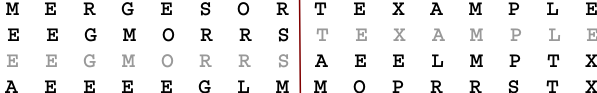
\includegraphics[scale=0.3]{figures/merge.png}

\smallskip

\tiny merge sort
\end{center}
\end{frame}

\begin{frame}[fragile]
\begin{framed}
\tiny merge.py: Reads strings from standard input, sorts them into increasing order, and writes them to standard output.
\end{framed}

\begin{lstlisting}[language=Python]
import stdarray
import stdio
import sys

def _merge(a, lo, mid, hi, aux):
    n = hi - lo
    i = lo
    j = mid
    for k in range(n):
        if i == mid:
            aux[k] = a[j]
            j += 1
        elif j == hi:
            aux[k] = a[i]
            i += 1
        elif a[j] < a[i]:
            aux[k] = a[j]
            j += 1
        else:
            aux[k] = a[i]
            i += 1
    a[lo:hi] = aux[0:n]
\end{lstlisting}
\end{frame}

\begin{frame}[fragile]
\begin{lstlisting}[language=Python]
def _sort(a, lo, hi, aux):
    n = hi - lo
    if n <= 1:
        return
    mid = (lo + hi) // 2
    _sort(a, lo, mid, aux)
    _sort(a, mid, hi, aux)
    _merge(a, lo, mid, hi, aux)

def sort(a):
    n = len(a)
    aux = stdarray.create1D(n)
    _sort(a, 0, n, aux)

def main():
    a = stdio.readAllStrings()
    sort(a)
    for s in a:
        stdio.write(s + ' ')
    stdio.writeln()

if __name__ == '__main__':
    main()
\end{lstlisting}

\begin{lstlisting}[language={}]
$ more tiny.txt 
the and was his you tom but for had him
\end{lstlisting}

\begin{lstlisting}[language={}]
$ python merge.py < tiny.txt 
and but for had him his the tom was you 
\end{lstlisting}
\end{frame}

\begin{frame}[fragile]
\begin{framed}
\tiny frequencycount.py: Reads words from standard input, and writes the frequency counts of the words to standard output.
\end{framed}

\begin{lstlisting}[language=Python]
import stdio
import sys
from counter import Counter

def main():
    words = stdio.readAllStrings()
    words.sort()
    zipf = []
    for i in range(len(words)):
        if (i == 0) or (words[i] != words[i - 1]):
            entry = Counter(words[i], len(words))
            zipf += [entry]
        zipf[len(zipf) - 1].increment()
    zipf.sort()
    zipf.reverse()
    for entry in zipf:
        stdio.writeln(entry)

if __name__ == '__main__':
    main()
\end{lstlisting}

\begin{lstlisting}[language={}]
$ python frequencycount.py < tomsawyer.txt
the: 3452
and: 2908
a: 1758
to: 1741
of: 1539
was: 1124
in: 926
...
\end{lstlisting}
\end{frame}
\end{document}
